\begin{frame}
  \frametitle{System}
  \begin{itemize}
    \item Homogeneous base stations, mmWave, downlink transmission, OFDMA, multiple-input eMBB and single-input URLLC users.
    \item Saturated eMBB traffic \cite{S05}: Each eMBB user has \highlight{infinite} amount of data to be served.
    \item Strict URLLC constraint: Each URLLC has an amount of data required to be served within a minislot.
    \item The system aims to maximize eMBB total average rate and fairness while satisfying URLLC demands.
  \end{itemize}
\end{frame}

\begin{frame}
  \frametitle{Scenario}
  \begin{itemize}
    \item There are approximately $750$ people per $1000$ square meters living in suburban area\exampleFootnote \cite{F19}.
    \item These are potential eMBB users, who surf the Web, watching videos, and download data.
    \item During work hours and at night, only a few self-driving vehicles operate that employ URLLC utilities.
      \begin{itemize}
        \item Uplink transmission (whose bandwidth is independent from that of downlink) is used to upload the vehicles' observations e.g. camera images, sensors data, etc. to the cloud for navigation processing.
        \item \highlight{Downlink} transmission accounts for the automobiles' control messages.
      \end{itemize}
  \end{itemize}
\end{frame}

\section{Issues and Solutions}
\subsection{Poor Edge Service}
\begin{frame}
  \frametitle{Poor Edge Service}
  \begin{itemize}
    \item Since mmWave is extremely vulnerable to path loss, URLLC reliability is not guaranteed.
    \item Similarly, eMBB users at cell edges experience low throughput.
  \end{itemize}
\end{frame}

\begin{frame}
  \begin{itemize}
    \item URLLC multicell and eMBB multiconnectivity are prominent candidates to mitigate this issue.
  \end{itemize}
\end{frame}

\begin{frame}
  \frametitle{Singlecell}
  \begin{figure}
    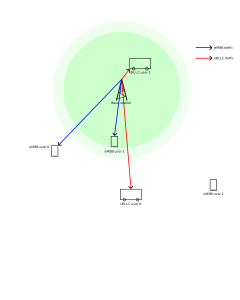
\includegraphics[width=0.6\textwidth]{model_singlecell}
    \caption{Singlecell model}
  \end{figure}
\end{frame}

\begin{frame}
  \begin{figure}
    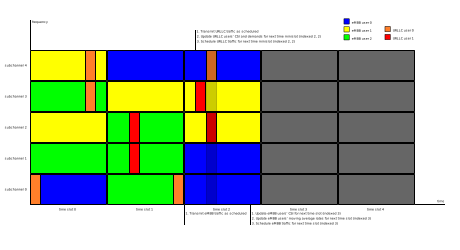
\includegraphics[width=1.05\textwidth]{framework_singlecell}
    \caption{Singlecell framework}
  \end{figure}
\end{frame}

\begin{frame}
  \frametitle{Multicell}
  \begin{figure}
    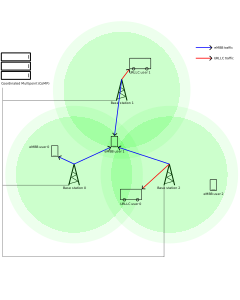
\includegraphics[width=0.6\textwidth]{model_multicell}
    \caption{Multicell model}
  \end{figure}
\end{frame}

\begin{frame}
  \begin{figure}
    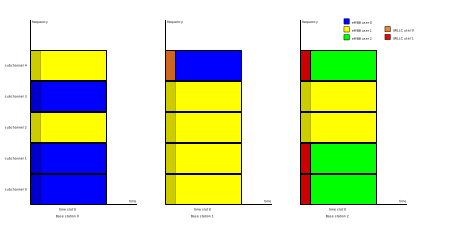
\includegraphics[width=1.05\textwidth]{framework_multicell}
    \caption{Multicell framework}
  \end{figure}
\end{frame}

\subsection{Multicell Co-channel Intereference}
\begin{frame}
  \frametitle{Multicell Co-channel Interference}
  \begin{itemize}
    \item Since the base stations are homogeneous i.e. use the same frequency band, there exists 3 types of interference:
      \begin{itemize}
        \item eMBB-eMBB inteference e.g. at subchannel $3$, signal from base station $0$ to eMBB user $0$ interferes with that from base station $1$ to eMBB user $1$.
        \item eMBB-URLLC interference e.g. at subchannel $0$, signal from base station $0$ to eMBB user $0$ interferes with that from base station $2$ to URLLC user $1$.
        \item URLLC-URLLC interference e.g. at subchannel $4$, signal from base station $1$ to URLLC user $0$ interferes with that from base station $2$ to URLLC user $1$.
      \end{itemize}
  \end{itemize}
\end{frame}

\begin{frame}
  \begin{itemize}
    \item A viable solution might be 5G Non-orthogonal Multiple Access (NOMA) with Successive Interference Cancellation (SIC). % TODO example
    \item Inspired by Low-Energy Adaptive Clustering Hierarchy (LEACH), we propose an orthogonal multiple access (OMA) scheme based on 3G Code Division Multiple Access (CDMA) to tackle the problem\exampleFootnote.
  \end{itemize}
\end{frame}

\begin{frame}
  \begin{itemize}
    \item Our scheme works well with the often small number of base stations.
    \item Our scheme encompasses URLLC \highlight{multiconnectivity} via joint transmission.
    \item This hence introduces a joint CDMA/OFDMA scheme.
  \end{itemize}
\end{frame}

\subsection{Spectrum Inefficiency}
\begin{frame}
  \frametitle{Spectrum Inefficiency}
  \begin{itemize}
    \item Dedicated URLLC bandwidth wastes spectral resources significantly in multicell systems.
      \begin{itemize}
        \item If $2$ subchannels of each base station are dedicated to URLLC traffic, then we would have $6$ subchannels sitting \highlight{idle for most of the time} in the aforementioned scenario.
      \end{itemize}
  \end{itemize}
\end{frame}

\begin{frame}
  \begin{itemize}
    \item This problem can be addressed by leveraging URLLC superposition/puncturing scheme. % TODO citations
    \item URLLC superposition scheme employs 5G NOMA SIC, whose performance equals to puncturing when the considered eMBB and URLLC users have the same channel gain. % TODO citations and example
    \item URLLC puncturing scheme is discussed here.
  \end{itemize}
\end{frame}
